\documentclass[12pt]{article}
\usepackage{paper,math}
\input{titlepage} 

% Set thesis information
\thesistitle{My Amazing Thesis Title}
\thesisauthor{Name Lastname}
\advisor{Dr. Jane Professor}
\department{Economics}
\departmentprefix{Department of}
\thesisdate{\today}
\thesisacknowledgements{%
  Email: \href{mailto:name@lastname.com}{name@lastname.com} \textcolor{red}{(use an email that will be accessible after graduation)..} I would like to thank my advisor and family...
}

\hypersetup{
  pdftitle = {My Amazing Thesis Title},
  pdfauthor = {John Smith},
}

% Conditionally display thoughts
\booltrue{INCLUDECOMMENTS}

%%%%%%%%%%%%%%%%%%%%%%%%%%%%%%%%%%
\begin{document}
%%%%%%%%%%%%%%%%%%%%%%%%%%%%%%%%%%

% Page 1: Thesis title page (no abstract) -- enter information above
\makethesistitle

%%%%%%%%%%%%%%%%%%%%%%%%%%%%%%%%%%
% Page 2: Academic format with title, author, and abstract  
\makeacademicpage
\noindent This is the abstract of my thesis. Lorem ipsum dolor sit amet, consectetur adipiscing elit, sed do eiusmod tempor incididunt ut labore et dolore magna aliqua. Ut enim ad minim veniam, quis nostrud exercitation ullamco laboris nisi ut aliquip ex ea commodo consequat.

\par\vspace{4em}\noindent
{\color{zinc700}Keywords:} machine learning, algorithms, optimization
\par\noindent
{\color{zinc700}JEL-Classification:} C61, C63
%%%%%%%%%%%%%%%%%%%%%%%%%%%%%%%%%%

\newpage

% Paper ------------------------------------------------------------------------
% ------------------------------------------------------------------------------
\section{Introduction}
% ------------------------------------------------------------------------------

Use of latex, rather than Word, is highly recommended for your thesis. Here is a short summary of their comparison and the advantages of latex: 

\href{https://blog.orvium.io/latex-over-word/}{https://blog.orvium.io/latex-over-word/}

You have the option to keep using Word, but you have to follow the same format (next section) as this template. Also, all thesis must have the first two title pages in the same way regardless of the writing software used.

\begin{itemize}
  \item This template is adapted from Kyle Butt's template available in 
  \href{https://github.com/kylebutts/latex-templates}{https://github.com/kylebutts/latex-templates}
  which also provides a latex beamer template for slides. 
  \item The other file in this folder, \texttt{thesistemplate.tex}, is a simple version with only a skeleton structure. 
  
  \texttt{titlepage.tex} is used in the template to insert the title page and academic page, and is not designed to be compiled on its own. All the information in pages 1 and 2 are set in the preamble of main .tex file. \texttt{paper.sty} is a style file that has a set of packages and commands that are useful for writing papers. Note that both style files (\texttt{paper.sty} and \texttt{math.sty}) need to be in the same folder as this main.tex file.\footnote{The file \texttt{math.sty} has a set of useful math operators. Credit to \url{https://pascalmichaillat.org/d3/}.}
  \item the bibliography file \texttt{references.bib} is in BibTex format. You can export your references from Google Scholar, Zotero, Mendeley, or other reference management software in BibTex format and add them to this file. It's loaded at the end by the \texttt{bibliography} command.
  \item To keep things organized, I recommend you create folders named \texttt{figures} and \texttt{tables} to store your figures and tables, respectively. You can then call them from that path when needed. See below for examples.
\end{itemize}


\bigskip

To get this all going, you need a latex compiler and a latex editor. For Mac, I recommend TexShop as an editor and MacTex as compiler free at \url{https://www.tug.org/mactex/}. Visual Studio Code also works, or you can do it online via Overleaf where you have UVA license: go to \url{https://www.overleaf.com/}, start a project, and upload all the contents of this folder. You don't need to download and install any compiler and editor, and can access it from any computer! 

Overleaf also has a very good tutorial for beginners:

\url{https://www.overleaf.com/learn/latex/Learn_LaTeX_in_30_minutes}


\subsection{Format and Margins}

The paper is set to 12pt Sans-serif font, with 1.5 line spacing, and 1 inch margins. Do not temper with these defaults. You can personalize some aspects of the style file, but do not change the margins, font character, font size, or line spacing.

\subsection{Some Commands}

See below for \autoref{thm:residue_thm}, the regression specification (\ref{eq:fe_reg}), \autoref{tab:summ_stat}, \autoref{fig:event_timing}, appendix \autoref{tab:reg1}. Of course, make sure to touch up on your micro theory with \cite{mas1995microeconomic}. 

Let's cite something in parenthesis: \citep{cosar2019}, or multiple people in parenthesis, as in: \citep{mas1995microeconomic, cosar2019}

You can make a word bold with \textbf{bold text} or italicized with \textit{italicized text}.

\subsection{Compiling}
If you use your own compiler, getting the references and links to sections and equations to work requires multiple compilations. If you use Overleaf, it does this automatically for you. 

In some compilers, you may need to run the following commands in sequence: first, run \texttt{pdflatex} to compile the main document, then run \texttt{bibtex} to compile the bibliography, and finally run \texttt{pdflatex} twice to ensure that all references and links are correctly updated.

% ------------------------------------------------------------------------------
\section{Highlights}
% ------------------------------------------------------------------------------

% ------------------------------------------------------------------------------
\subsection{Math Commands}
% ------------------------------------------------------------------------------

Theorem environment: there are the following environments: \texttt{theorem}, \texttt{proposition}, \texttt{assumption}, \texttt{example}, \texttt{lemma}, \texttt{corollary}, \texttt{definition}, \texttt{remark} -- may not be super relevant for empirical work though. 

\begin{theorem}[Example Theorem]\label{thm:residue_thm}
  This is an example theorem \[
    \hat{\beta}=\frac{\sum_{\ell}e_{\ell}z_{\ell}y_{\ell}^{\perp}}{\sum_{\ell}e_{\ell}z_{\ell}x_{\ell}^{\perp}}
  \]
\end{theorem}

Jibberish math to show off symbols:

\begin{equation}\label{eq:fe_reg}
  y = f(X) + \varepsilon = X \beta + \psi_i + \nu_t + w_{i,t} + \varepsilon_{i,t}
\end{equation}

When you use the \texttt{equation} command, you get numbered equations that you can label and refer to such as equation \ref{eq:fe_reg} -- as you change things, this updates automatically.

The command \$\$ \$\$ with math in between creates unnumbered equations, as does this: 

\begin{equation*}
y=x
\end{equation*}

The command \$ \$ creates in line math: $y=z$

\bigskip

\texttt{\textbackslash one} does an indicator (dummy variables!): 

$$\one{X_i > 0}$$



% ------------------------------------------------------------------------------
\subsection{Tables}
% ------------------------------------------------------------------------------

For tables, I use the \texttt{tabular} and \texttt{booktabs} packages. For table and figure notes, I use a custom \texttt{\textbackslash note} command. It uses \texttt{\textbackslash parbox} under the hood. You can use it in one of of four ways:
\begin{enumerate}
  \item \texttt{\textbackslash note\{text\}}
  \item \texttt{\textbackslash note[Notes.]\{text\}}
  \item \texttt{\textbackslash note\{0.6\textbackslash textwidth\}\{text\}}
  \item \texttt{\textbackslash note[Notes.]\{0.6\textbackslash textwidth\}\{text\}}
\end{enumerate}

In addition, I use the \texttt{adjustbox} package for resizing figures/tables. It automatically scales the figure/table proportionally, so things look right. For example, here's a table that's too wide. I use the \texttt{adjustbox} package to fix it.

\begin{table}[ht]
  \caption{Table Too Wide (adjustbox)}\label{tab:summ_stat}
  \centering

  \begin{adjustbox}{width = \textwidth, center}
    \begin{tabular}{ 
      @{} @{\extracolsep{5pt}} l*{8}{r} @{}
    }
      % Head
      \toprule
      & & & \multicolumn{2}{c}{Market Access} & \multicolumn{2}{c}{Urban Weekly Wage} & \multicolumn{2}{c}{Nonurban Weekly Wage} \\
      \cmidrule{4-5} \cmidrule{6-7} \cmidrule{8-9}
      Year & \multicolumn{1}{c}{N} & \% Urban & Mean & SD & Mean & SD & Mean & SD \\
      \hline

      % Body
      \input{tables/summary.tex}

      \bottomrule
    \end{tabular}
  \end{adjustbox}

  \note{Weekly wage is reported in 2015.}
\end{table}

Figures also use the \texttt{\textbackslash note} and the \texttt{adjustbox} package. Here's an example figure:

\begin{figure}[h!]
  \caption{Event-timing}\label{fig:event_timing}
  \begin{adjustbox}{width = 0.6\textwidth, center}
    \begin{tikzpicture}
      \draw (0,0) -- (11,0);
      \foreach \x in {0.8,4,5.5,7,10.2}
      \draw(\x cm,3pt) -- (\x cm, -3pt);
      \draw (0.8,0) node[below=3pt] {$T_0$};
      \draw (4,0) node[below=3pt] {$T_1$};
      \draw (5.5,0) node[below=3pt] {$0$};
      \draw (7,0) node[below=3pt] {$T_2$};
      \draw (10.2,0) node[below=3pt] {$T_3$};
      \draw (2.35,0) node[above=6pt, align=center]
      {\begin{tabular}{c}Estimation \\Window\end{tabular}};
    \end{tikzpicture}
  \end{adjustbox}
  
  \begin{center}
    \note{0.6\textwidth}{This is an example figure in the paper}
  \end{center}
\end{figure}

In practice, \texttt{tikzpicture} environment is not super important for your purposes but it has conveniences depending on the need. You will mostly use:

\begin{verbatim}
\begin{figure}[htbp]
    \centering
    %\includegraphics[width=0.8\textwidth]{graph.pdf}
    \caption{This is the figure caption describing what the figure shows.}
    \label{fig:example}
\end{figure}
\end{verbatim}

\noindent [remove the verbatim commands to make this a real command that renders \texttt{graph.pdf} file] You display the file titled \texttt{graph.pdf} with the appropriate path structure, i.e., it can be in a folder titled \texttt{figures} and used as 

\begin{verbatim}
\includegraphics[width=0.8\textwidth]{figures/graph.pdf}
\end{verbatim}

For example:

\begin{figure}[htbp]
    \centering
    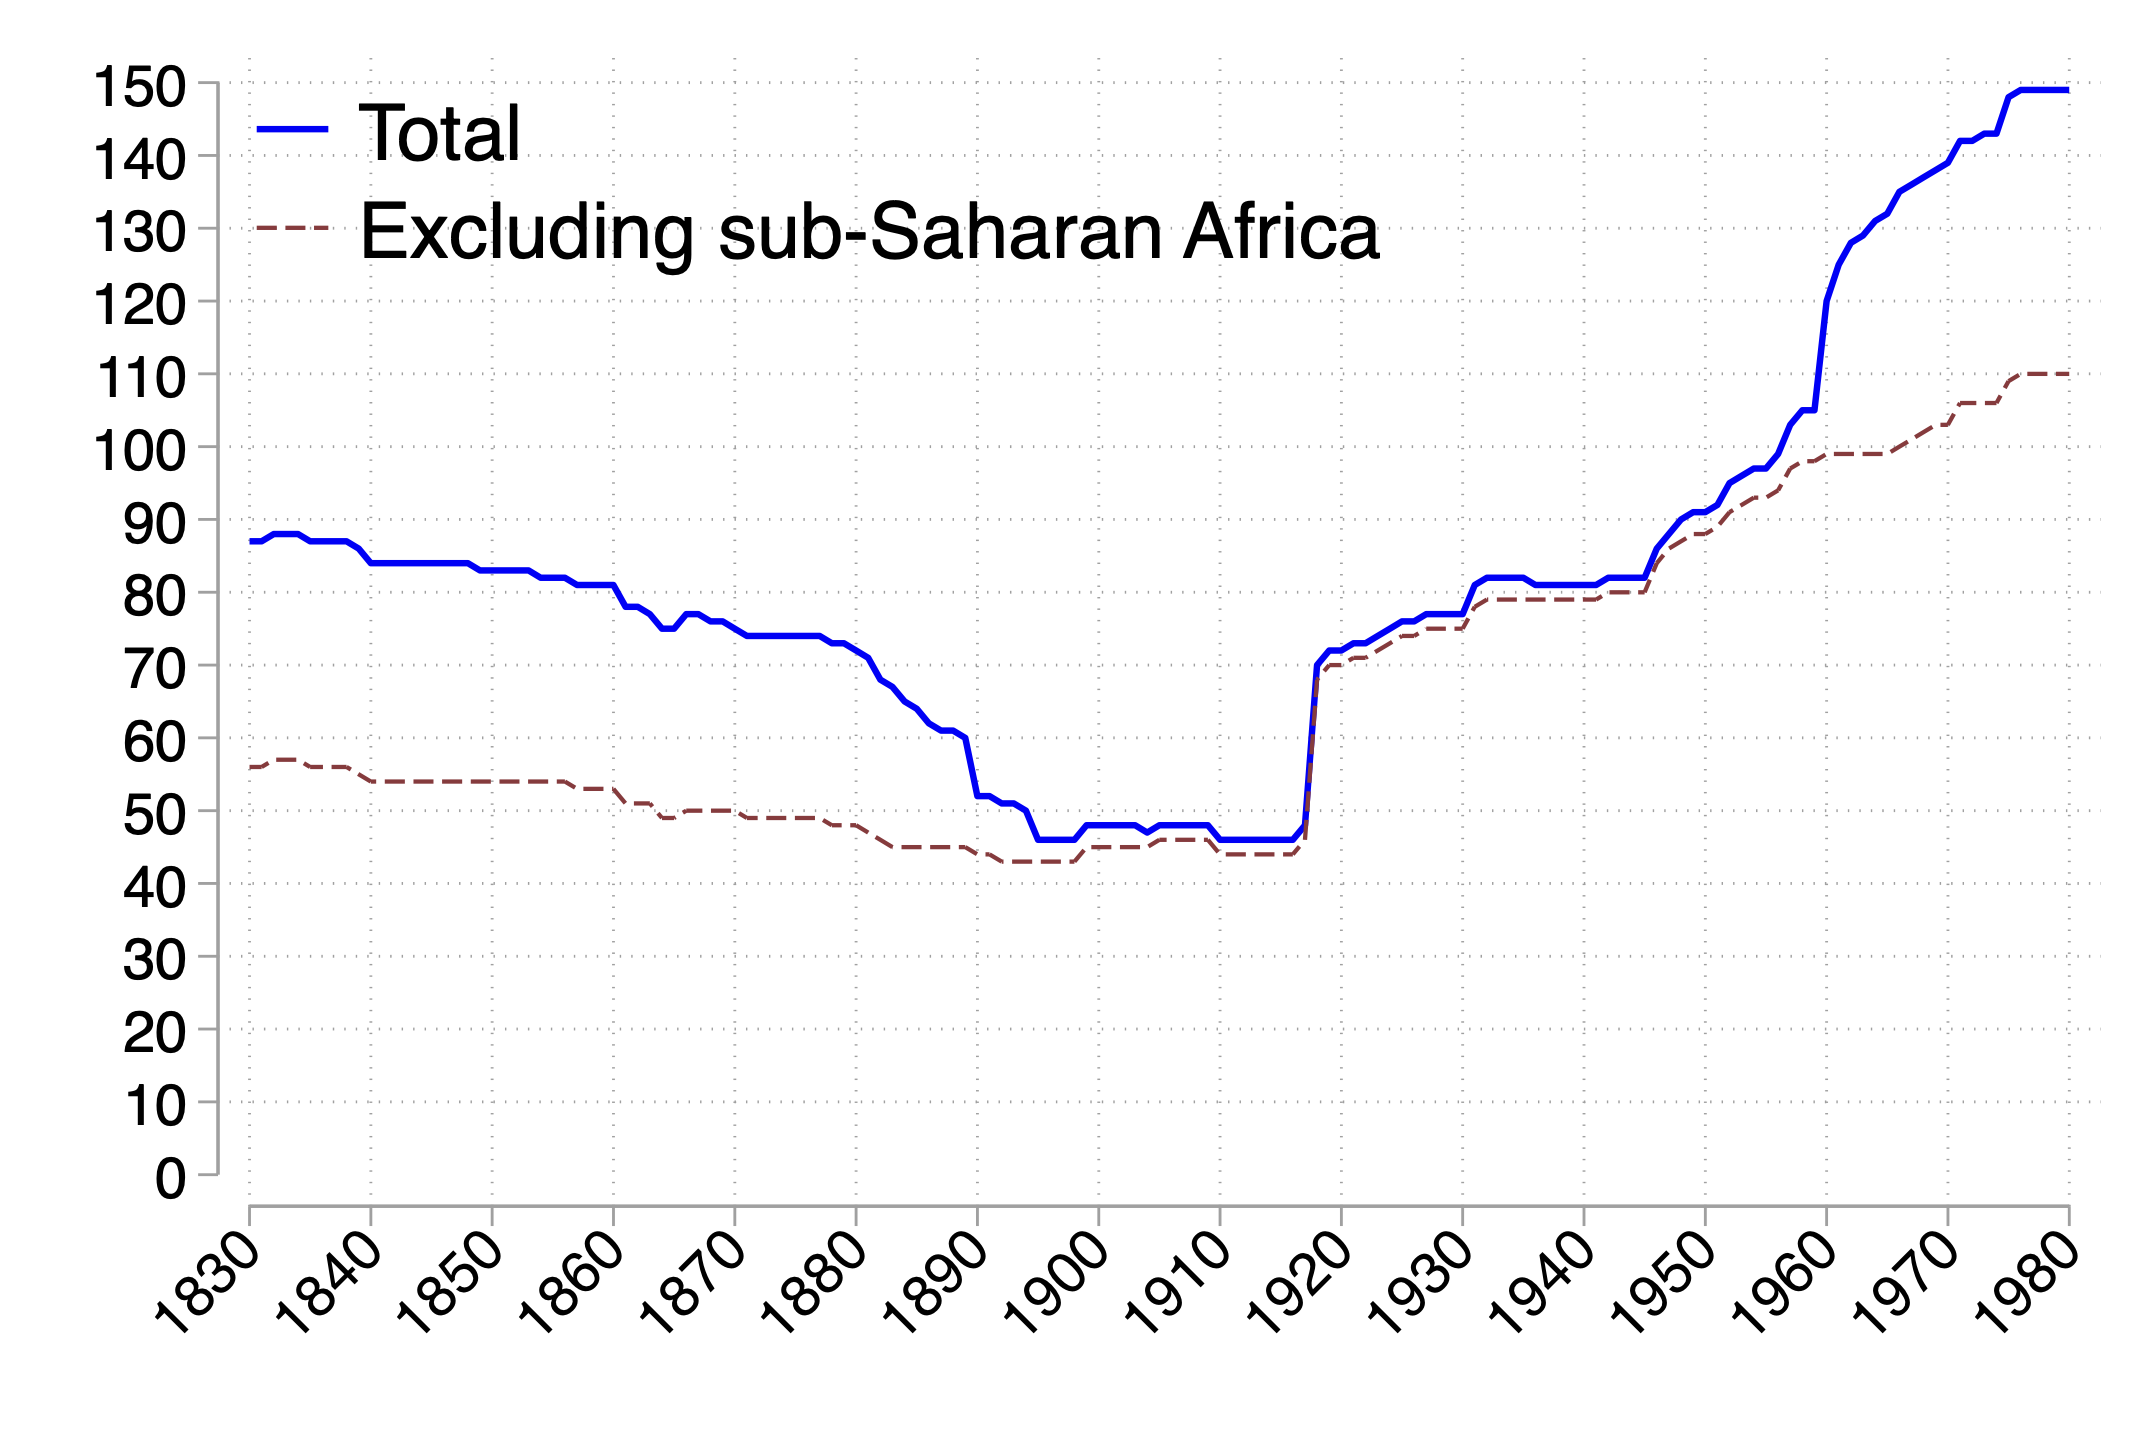
\includegraphics[width=1\textwidth]{figures/figure1}
    \caption{This is the figure caption describing what the figure shows.}
    \label{fig:example2}
\end{figure}

% ------------------------------------------------------------------------------
\clearpage
\bibliography{references} 
% ------------------------------------------------------------------------------

% ------------------------------------------------------------------------------
\newpage~\appendix
% ------------------------------------------------------------------------------

% ------------------------------------------------------------------------------
\section{Additional Results}
% ------------------------------------------------------------------------------

The appendix will automatically start numbering tables, figures, and theorem-like environments using the appendix section \textbackslash Alph (e.g. \autoref{tab:reg1}).

You can still cite \cite{mas1995microeconomic} 

% ------------------------------------------------------------------------------
\subsection{Regression Results}
% ------------------------------------------------------------------------------

The main regression equation is 
\begin{equation}
  y_i = \bm{X}_i \beta + u_i.
\end{equation}

Results are presented in \autoref{tab:reg1}. In this table example, the table is narrower than textwidth, so I adjust the \texttt{\textbackslash note} width. 

\begin{table}[h!]
  \caption{Regression Results}
  \label{tab:reg1}
  \begin{center}
    \begin{tabular}{@{} lrr @{}}
      % Head
      \toprule
      & \multicolumn{2}{c}{\textit{Dependent variable:} \ Overall Rating} \\
      \cmidrule{2-3}
                                & (1)                   & (2)                   \\
      \hline

      % Body
      Handling of Complaints   & 0.692$^{***}$ (0.149) & 0.682$^{***}$ (0.129) \\
      No Special Privileges    & $-$0.104 (0.135)      & $-$0.103 (0.129)      \\
      Opportunity to Learn     & 0.249 (0.160)         & 0.238$^{*}$ (0.139)   \\
      Performance-Based Raises & $-$0.033 (0.202)      &                       \\
      Too Critical             & 0.015 (0.147)         &                       \\
      Advancement              & 11.011 (11.704)       & 11.258 (7.318)        \\
      \hline
      Observations             & 30                    & 30                    \\
      Adjusted R$^{2}$         & 0.656                 & 0.682                 \\

      \bottomrule
    \end{tabular}

    \note{0.68\textwidth}{Using R base dataframe attitude. dolor in reprehenderit in voluptate velit esse cillum dolore eu fugiat nulla pariatur. Excepteur sint occaecat cupidatat non proident, sunt in culpa qui officia deserunt mollit anim id est laborum.}
    \note[]{0.68\textwidth}{$^{*}$ $p < 0.1$; $^{**}$ $p < 0.05$; $^{***}$ $p < 0.01$.}
  \end{center}
\end{table}


\end{document}
